А) Дано пространство геометрических векторов  $\mathbb{R}^3$, его подпространства  $L_1$  и  $L_2$  и линейный оператор  $\mathcal{A}:\ \ \mathbb{R}^3\rightarrow\mathbb{R}^3$.
Проведите исследование:
\begin{enumerate}
    \item Изобразите на графике подпространства  $L_1$  и  $L_2$.
    \item Методами векторной алгебры составьте формулу для линейного оператора  $\mathcal{A}$.
    \item Составьте его матрицу в базисе $\left\{\vec{i},\vec{j},\vec{k}\right\}$ пространства $\mathbb{R}^3$.
    \item Решите задачу о диагонализации полученной матрицы методом спектрального анализа.
    \item На построенном ранее графике изобразите базис, в котором матрица линейного оператора $\mathcal{A}$ имеет диагональный вид. Объясните его смысл.
\end{enumerate}

$\mathcal{A}$ – оператор отражения пространства  $\mathbb{R}^3$ в $L_1$ параллельно $L_2,$ где $L_1$ задано уравнением $x=0$, $L_2$ – уравнением  $2x=y=-z$.

\vspace{10mm}

\textbf{Решение.}

\begin{enumerate}
    \item Графики подпространства

    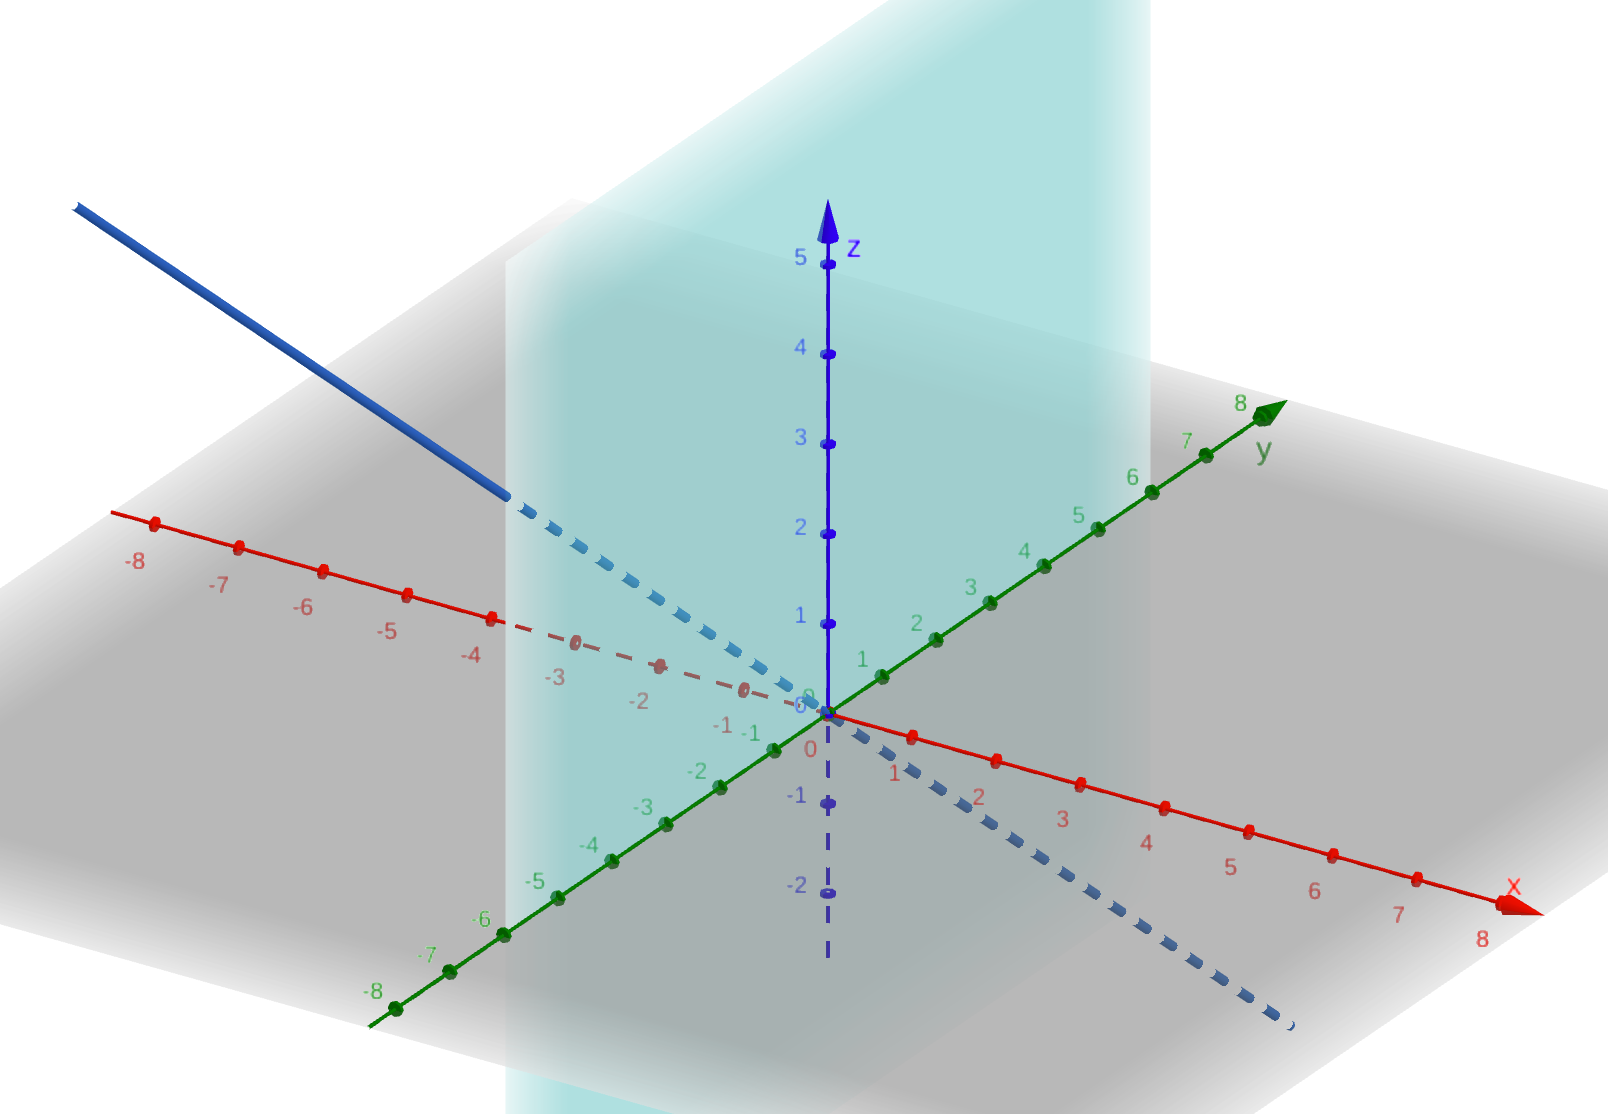
\includegraphics[scale=0.15]{images/3a2_1}
    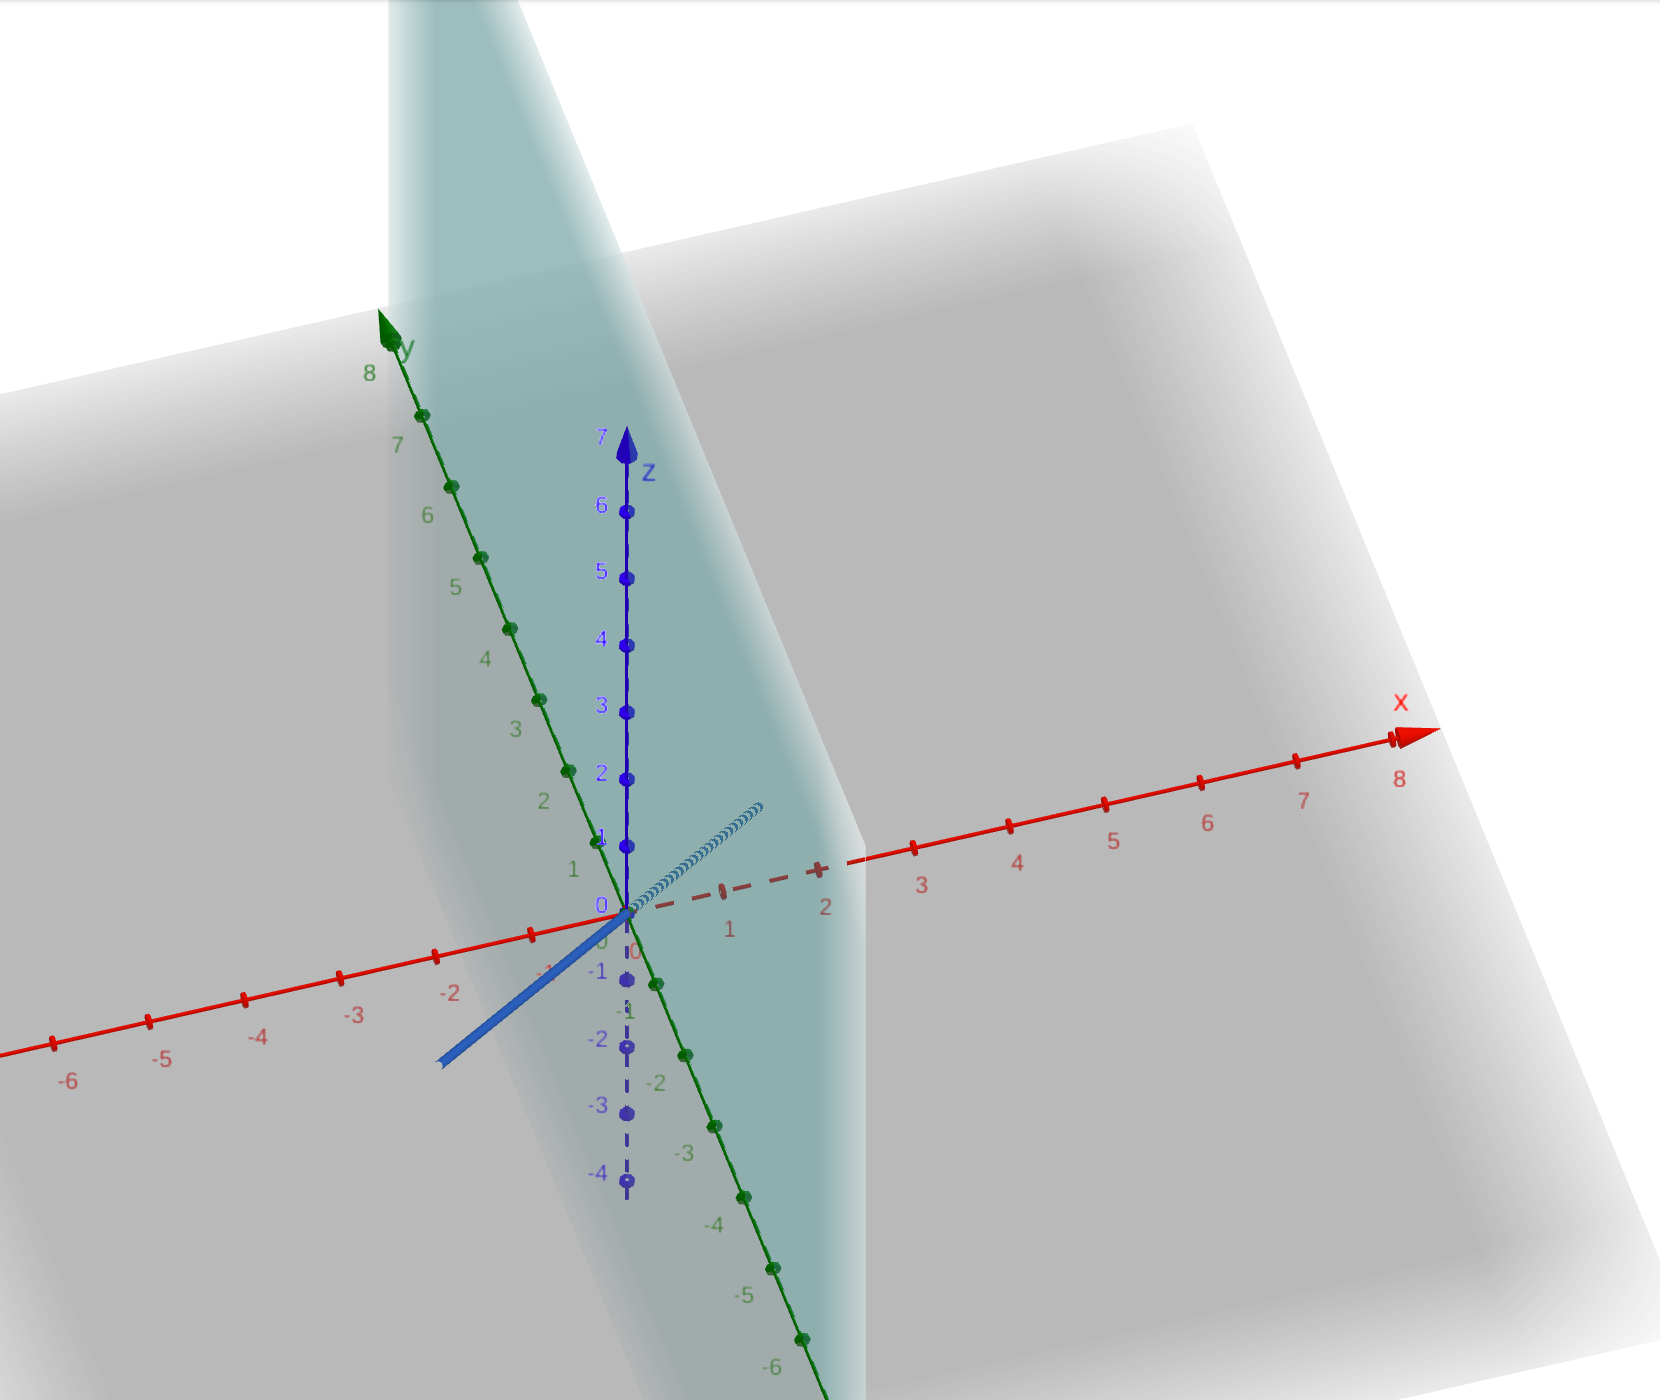
\includegraphics[scale=0.15]{images/3a2_2}

    \item Формула для линейного оператора

    Отражение через $Oyz$ параллельно прямой значит что нам надо пройти через $Oyz$ по $x$ в другую сторону на $x$.
    Т.е. сделать $x=-x$.
    И также поправить все другие координаты. Как? По нужной прямой, параллельной $2x=y=-z$.

    Чтобы ее построить можно задать прямую проходящую через нашу точку в $\mathbb{R}^3$. Т.е. $2(x-x_0)=(y-y_0)=-(z-z_0)$.
    Т.е. нам надо прибавить какой-то вектор параллельный нашей прямой.

    Когда мы проходим расстояние $x=1$ то $y$ и $z$ меняются на $2$.
    Т.е. наш вектор $x = \Set{1, 2, -2}$.
    Этот вектор нужно умножить на два и вычесть из нашего вектора
    (если мы просто вычтем этот вектор из данного, мы окажемся в плоскости $x=0$).

    Т.е. $\mathcal{A}: \mathbb{R}^3 \rightarrow \mathbb{R}^3$ задает перемещение и выглядит: $\mathcal{A}x = x - \Set{1,2,-2} * 2 * (x, i)$,
    где $(x,i)$ - скалярное произведение (необходимое для нахождения координаты $x$).

    \item Линейный оператор

    Запишем, как должна меняться каждая координата при применении оператора:

    (мы знаем что $x$ меняет знак, а все остальные координаты можно найти через уравнение прямой)

    \begin{equation*}
        \begin{cases}
            $x' = -x$\\
            $y' = 2(x'-x) + y$\\
            $z' = -2(x'-x) + z$
        \end{cases}
    \end{equation*}

    \begin{equation*}
        \begin{cases}
            $x' = -x$\\
            $y' = -4x + y$\\
            $z' = -4x + z$
        \end{cases}
    \end{equation*}

    \begin{equation*}
        \begin{cases}
            $x' = -x + 0y + 0z$\\
            $y' = -4x + y + 0z$\\
            $z' = 4x + 0y + z$
        \end{cases}
    \end{equation*}

    Как можно видеть:

    $ A =
    \begin{pmatrix}
        -1 & 0 & 0 \\
        -4 & 1 & 0 \\
        4  & 0 & 1
    \end{pmatrix}
    $

    \item Диагонализация

    Чтобы решить задачу диагонализации, найдем ортогональный базис из собственных векторов этой матрицы.

    $
    \begin{vmatrix}
        -1 - \lambda & 0           & 0           \\
        -4           & 1 - \lambda & 0           \\
        4            & 0           & 1 - \lambda
    \end{vmatrix}
    $
    $ = -(1+\lambda)
    \begin{vmatrix}
        1-\lambda & 0         \\
        0         & 1-\lambda
    \end{vmatrix}
    = -(1+\lambda)(1-\lambda)^2
    $\\

    Значит $\lambda = 1$ или $\lambda = -1$.

    \begin{enumerate}
        \item $\lambda = 1$

        $
        \begin{pmatrix}
            -2 & 0 & 0 \\
            -4 & 0 & 0 \\
            4  & 0 & 0
        \end{pmatrix} = 0.
        $
        Как видно $x = 0$ всегда должен быть, а что на $y,z$ вообще не важно.
        Для простоты возьмем $y = 1$ и $z = 1$. Т.е. эта система нам дает два вектора: $\Set{0,1,0}, \Set{0,0,1}$.

        \item $\lambda = -1$

        $
        \begin{pmatrix}
            0  & 0 & 0 \\
            -4 & 2 & 0 \\
            4  & 0 & 2
        \end{pmatrix} = 0.
        $
        $
        \begin{pmatrix}
            -4 & 0 & -2 \\
            0  & 2 & 2
        \end{pmatrix} = 0.
        $

        Как видно из системы: $-4x -2z = 0 \rightarrow x = -1/2z$,
        $2y+2z=0 \rightarrow y=-z$. Т.е. получаем один собственный вектор, который является ФСР данной системы: $\Set{-0.5z,-z,z}$, т.е. $\Set{-0.5,-1,1}$.

        \item Базис диагонализированного оператора

        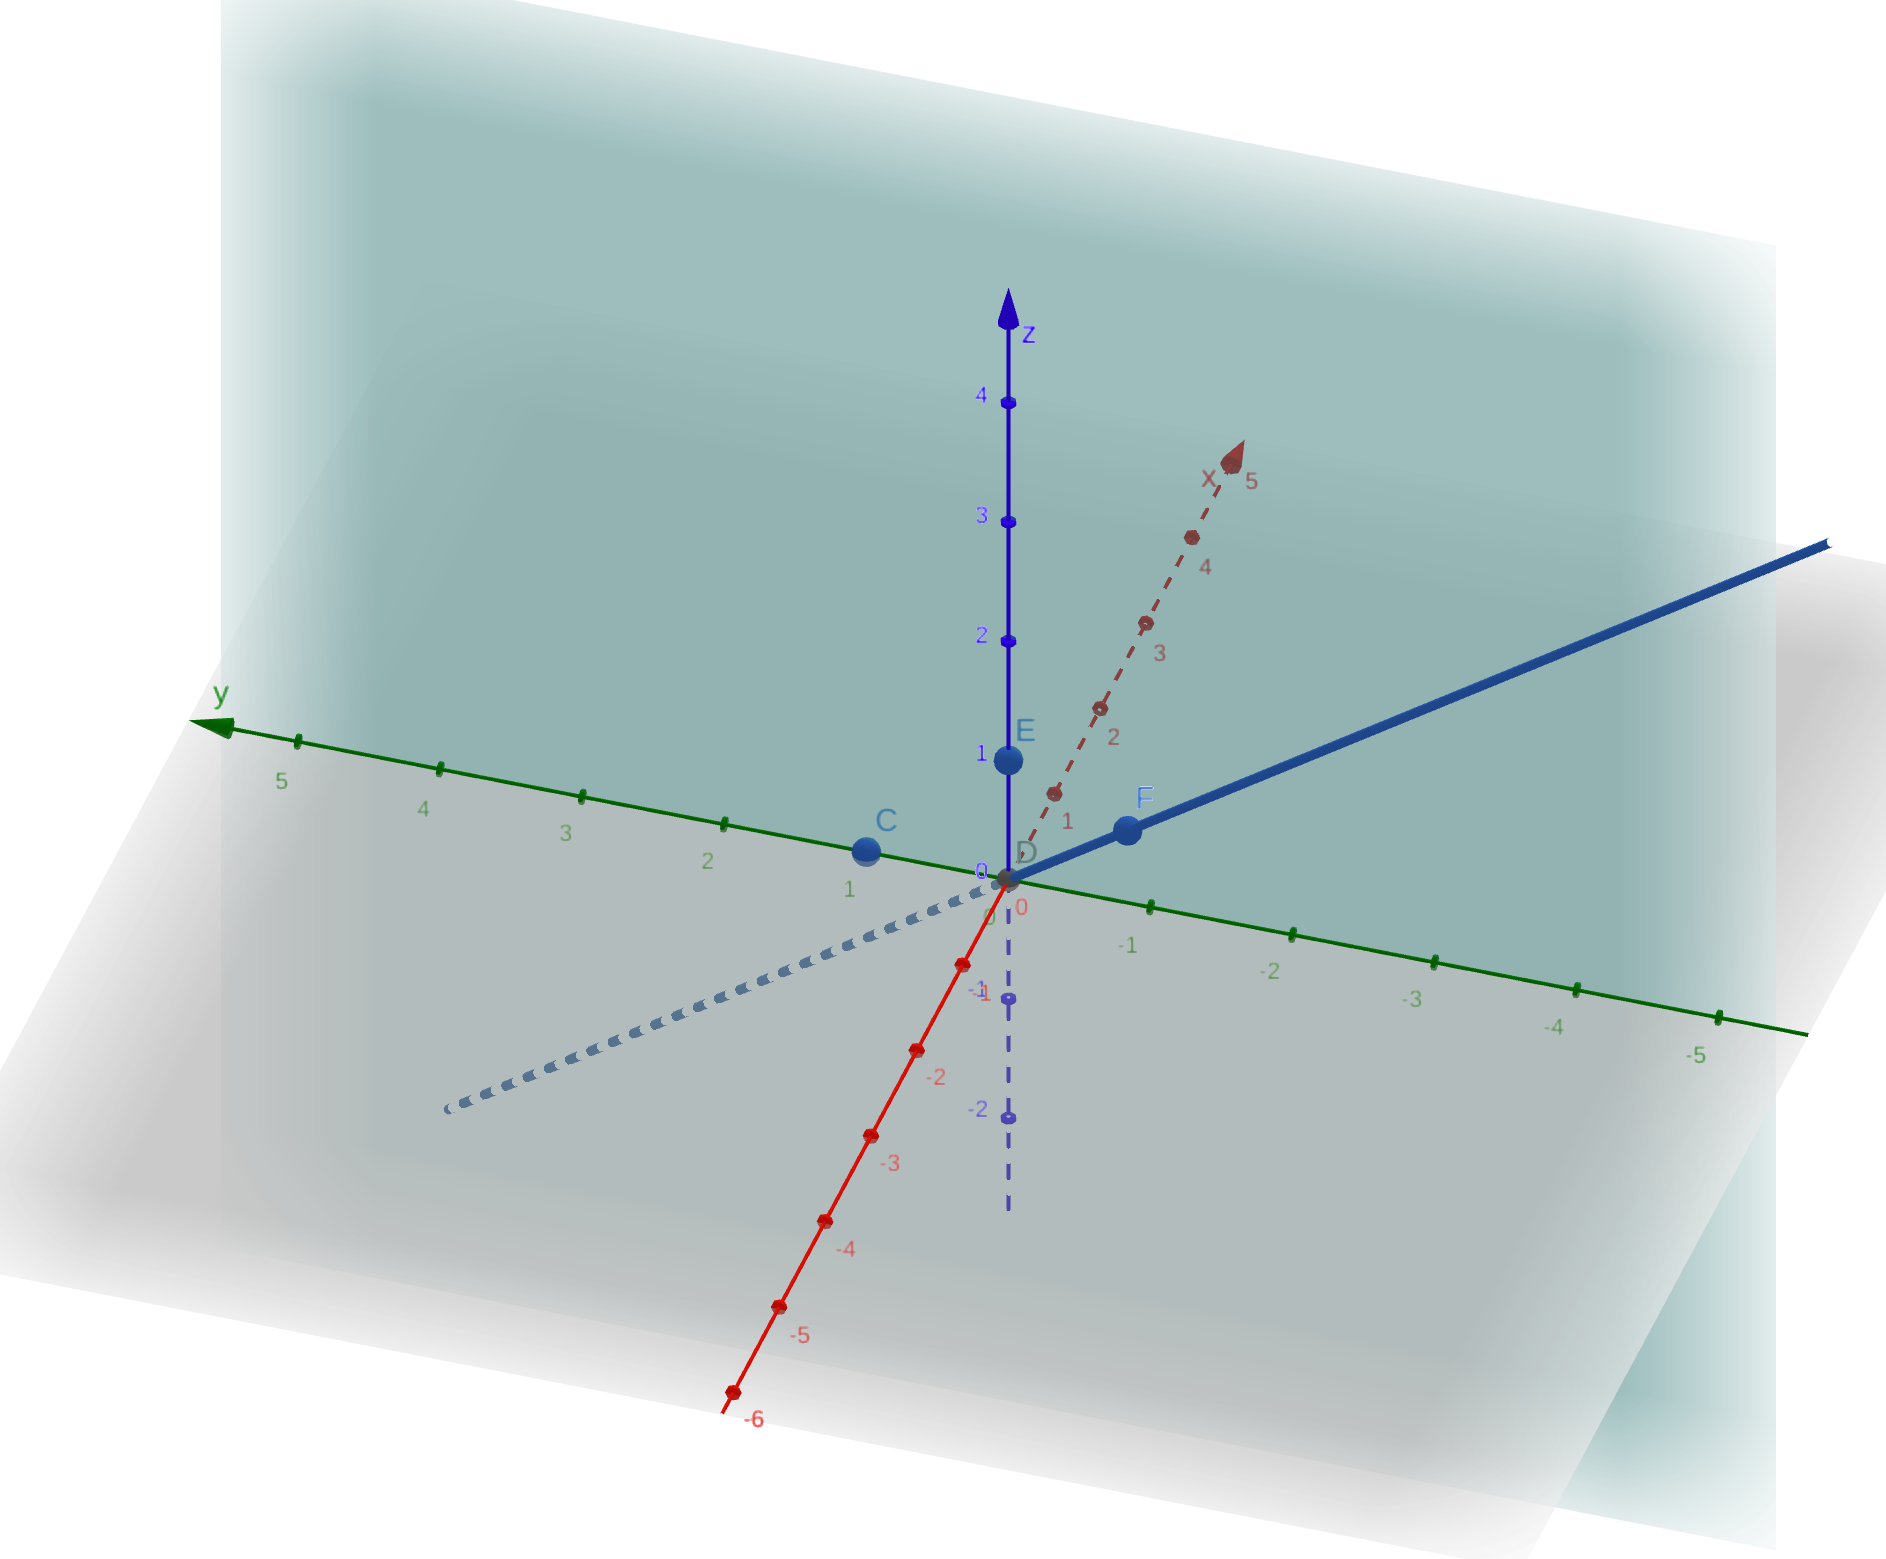
\includegraphics[scale=0.2]{images/3a5}

        Три вектора: $\overrightarrow{DC}, \overrightarrow{DE}, \overrightarrow{DF}$.
        Это соответственно вектора: $\Set{0,0,1}, \Set{0,1,0}, \Set{-0.5,-1.1}$. Первые два вектора буквально значат то, что мы можем перемещаться относительно $Oyz (y = 1, z = 1)$. Третий же вектор и означает то самое параллельное отражение относительно прямой $2x=y=-z$.

    \end{enumerate}

\end{enumerate}